
In this chapter we present the SMT problem. Recall that our goal is to translate proofs of unsatisfiability of SMT queries into Lean proofs. Therefore, besides presenting formally the problem and explaining how it is solved, we focus on showing how proofs are structured in an SMT solver.

\subsection{Description of the Problem}

The Boolean Satisfiability Problem (SAT) consists in, given a formula in Propositional Logic (PL) containing free variables, determining whether there exists a function that assigns each variable to a boolean value, in a way that, after replacing the variables by their values provided by the function, the formula is evaluated to \textit{true}. We say that a formula is satisfiable if such function exists, and unsatisfiable otherwise. In this work, we will be focusing on the problem CNF-SAT, an equivalent version of SAT in which the input formula always comes in Conjunctive Normal Form, that is, a conjunction of disjunctions. From now on, we will use SAT to refer to the CNF-SAT problem. Besides that, we will use the name \textit{clause} to refer to each one of the disjunctions in some input formula for SAT.

Satisfiability Modulo Theories (SMT)~\cite{smt} is a generalization of SAT.\ There are two additions in this version of the problem: the first one is that the input formula can contain quantifiers binding variables, which will affect the satisfiability of that formula. Therefore, any formula in First Order Logic is a valid input to the SMT problem. The second addition is the inclusion of a set of theories that allows the problem to refer to variables of different domains. More precisely, a theory consists of a sort (for instance, integers) over which a subset of the variables of the problem can range over and a set of symbols that represents operations over these sorts with predefined semantics (for instance, addition and comparison operations over integers). Instances of the problem are allowed to use multiple theories at the same time. The logic framework that corresponds to Propositional Logic with these two additions is known as Many-Sorted First Order Logic (MSFOL). The semantics of this logic are given in detail in~\cite{many_sorted}. In Section~\ref{sec:msfolHere} we give a brief overview of it.

\subsection{Many-Sorted First Order Logic}\label{sec:msfolHere}

The syntax of MSFOL can be described with three syntatic categories:

\begin{enumerate}
  \item \textbf{Sorts}. Symbols identifying the kinds of variables that are allowed. They are defined by the following grammar:
        \begin{center}
          $ \tau ::= \sigma \mid (\tau_{1}, \tau_{2}, \ldots, \tau_{n}) \rightarrow \tau \mid (\tau_{1}, \tau_{2}, \ldots, \tau_{m})$
        \end{center}
        Where the first case represents an atomic sort drawn from a set of predefined sorts, which we will refer to as $\mathcal{S}_{S}$, the second case represents functions with arity $n$ and the third case represents predicates of arity $m$.
  \item \textbf{Terms}. Symbols representing sorted variables, constants or function applications. Notice that function applications are only well formed when the sorts are respected. The symbols annotated on top of each term represent their sort, and they will be ommited when they can be inferred.
        \begin{center}
          $ t ::= x^{\tau} \mid f^{(\tau_{1}, \ldots, \tau_{n}) \rightarrow \tau}(t_{1}, \dots, t_{n}) $
        \end{center}
        Function symbols are drawn from a predefined set, which we will refer to as $\mathcal{S}_{F}$. Constants are represented by nullary functions.
  \item \textbf{Formulas}. Symbols representing boolean expressions, possibly involving terms. Predicate applications are also only well formed when the sorts are respected. They are drawn from a predefined set which we will refer to as $\mathcal{S}_{P}$.
        \begin{center}
          $ \psi ::= \bot \mid \psi_{1} \vee \psi_{2} \mid \forall x.\psi \mid \neg \psi \mid p^{(\tau_{1}, \ldots, \tau_{m})}(t_{1}, \dots, t_{m}) $
        \end{center}
\end{enumerate}

We also define the following symbols:

\begin{center}
  $\exists x. \psi := \neg \forall x. \neg \psi$\\
  $\psi_{1} \wedge \psi_{2} := \neg (\neg \psi_{1} \vee \neg \psi_{2})$\\
  $\psi_{1} \Rightarrow \psi_{2} := \neg \psi_{1} \vee \psi_{2}$\\
  $\psi_{1} \Leftrightarrow \psi_{2} := \psi_{1} \Rightarrow \psi_{2} \wedge \psi_{2} \Rightarrow \psi_{1}$
\end{center}

\begin{definition}[Theory]
  A theory $\mathcal{T}$ is a triple of sets $\langle \mathcal{S}_{S}, \mathcal{S}_{F}, \mathcal{S}_{P}\rangle$ together with a formal definition of the corresponding semantics, that is, for each function $f \in \mathcal{S}_{F}$, what is the resulting constant of applying $f$ to each possible sequence of arguments. Also, for each predicate $p \in \mathcal{S}_{P}$ and for each possible sequence of arguments, whether it is a tautology or not.
\end{definition}

\begin{example}[LIA]\label{ex:lia}
  Let $\mathcal{S}_{S} := \{\mathbb{Z}\}$, $\mathcal{S}_{F} := \{+, -, 0, succ, pred\}$ and $\mathcal{S}_{P} := \{<, \le, =, \ge, >\}$. Let's define the semantics of $+$ and $-$ as the usual semantics of addition and subtraction and multiplication over integers. $0$ is a nullary function representing the integer zero. $succ$ and $pred$ are unary functions representing successor and predecessor of integers. Also, let's define the semantics of $<$, $\le$, $=$, $\ge$ and $>$ as the usual semantics of comparison relations over integers. We denote by $\mathcal{T}_{LIA}$ (LIA standing for Linear Integer Arithmetic) the theory defined by $\langle \mathcal{S}_{S}, \mathcal{S}_{F}, \mathcal{S}_{P} \rangle$. An example of formula in this theory is $3x + 2y < 0 \vee 3x + 2y > 0$. Notice that we do not have a multiplication function in $\mathcal{S}_{F}$, so terms like $3x$ and $2y$ are abbreviations for $x + x + x$ and $y + y$.
\end{example}

\subsection{SMT Solvers}

An SMT solver is a piece of software whose main goal is to solve the SMT problem. Many-Sorted First Order Logic is undecidable in it's most general form~\cite{fol_undec}, therefore SMT solvers have to limit themselves to use heuristics to solve the a subset of the instances of the problem. In this section we present the ideas used by these systems that are most relevant to the present work.

\subsubsection{DPLL}

First, let’s explore how SAT is solved. Although MSFOL is not decidable, Propositional Logic is, therefore, it is possible to design a decision procedure for SAT.\@ Indeed, one simple way to check whether a formula in PL with $n$ variables is satisfiable or not is to simply test each one of the $2^{n}$ functions assigning truth values to those variables.

A more efficient alternative of a decision procedure for PL is the DPLL algorithm~\cite{dpll}. DPLL is based on the \textit{Resolution} theorem:

\begin{theorem}[Resolution]
Let $x$ be a literal. Let $C_{1}$ and $C_{2}$ be two clauses such that $x \in C_{1}$ and $\overline x \in C_{2}$. Then $C_{1} \wedge C_{2} \rightarrow (C_{1} \setminus x) \vee (C_{2} \setminus \overline x)$.
\end{theorem}

More specifically, it is based on \textit{Unit Resolution} (UR), that is, a more restricted version of Resolution in which $C_{1} = \{x\}$ or $C_{2} = \{\overline x\}$. We present DPLL's pseudocode and a brief explanation over it:

\begin{algorithm}[H]
\caption{DPLL Algorithm}~\label{dpllAlgo}
% \textbf{Input:} $\psi$, a PL formula\\
% \textbf{Output:} \textit{true} or \textit{false}, depending whether $\psi$ is satisfiable
\begin{algorithmic}[1]
\Function{SolvePL}{$\psi$}
\State $\psi \gets \Call{ConvertCNF}{\psi}$
\If{$\exists C \in \psi .\, C = \{\bot\}$}
  \State \Return~\textit{false}
\ElsIf{$\forall C \in \psi .\, \top \in C$}
  \State \Return~\textit{true}
\Else
  \If{$\exists x \in Vars(\psi) \,$ such that $x$ is a target for UR}
    \State $\langle C_{1}, C_{2} \rangle \gets$ \Call{findClauses}{$x$, $\psi$} \Comment{Clauses suitable for applying UR with $x$}
    \State~\Return~\Call{SolvePL}{$\psi \wedge C_{1} \diamond_{x} C_{2}$}
  \Else
    \State~Let $x$ be an unassinged variable in $\psi$
    \State~\Return~\Call{SolvePL}{$\psi_{\{x \gets \top\}}$} $\vee$ \Call{SolvePL}{$\psi_{\{x \gets \bot\}}$}
  \EndIf
\EndIf
\EndFunction
\end{algorithmic}
\end{algorithm}

The algorithm works as follows: first, it checks to see if the formula can be evaluated to \textit{true} or \textit{false}. In case it is not possible, the procedure finds as many variables in which it can apply Unit Resolution as possible, invoking itself recursively with each new application found. By the resolution theorem, the formula that will be used as a parameter in the recursive call is satisfiable if and only if the one that was received by input is also satisfiable, therefore, this step is sound. Once there are no more possibilities, it chooses an arbitrary variable and make two recursive calls: one assigning this variable to \textit{true} and the other one to \textit{false}. Since these are the only two possibilities for that variable, the input formula is satisfiable if and only if one of the recursive calls returned \textit{true}. The algorithm uses this information to correctly return the disjunction between the two return values.

The actual algorithm used by most SMT solvers is a refinement over DPLL, called CDCL~\cite{cdcl}.\ Since this refinement is not relevant for this work, we will not present it here.

\subsubsection{DPLL(T)}

Assuming that we have a decision procedure for a given theory (or a combination of them), we can use it to extend the DPLL algorithm for checking the satisfiability of MSFOL formulas involving that theory. In this section we will study the DPLL(T) framework, that is a method for doing this extension over DPLL. The actual strategy used by SMT solvers is known as CDCL(T), which is analogous to DPLL(T), except that it is an extension over CDCL instead of DPLL.

Consider a formula $\psi$ over a theory $\mathcal{T}$ in MSFOL.\ Let's assume we have a solver for this theory (that is, a method for deciding whether a given set of propositions in $\mathcal{T}$ is consistent or not). The idea behind DPLL(T) is to create a PL formula $\psi'$ from $\psi$ by substituting each term in it for a fresh boolean variable. We can then use the previously described DPLL algorithm to determine whether $\psi'$ is satisfiable. If it is unsatisfiable, then $\psi$ is also unsatisfiable. Otherwise, we can find a model $M$ for $\psi'$. Although $M$ satisfies $\psi'$, it is possible that it contradicts some fact about $\mathcal{T}$. For instance, consider $\psi$ to be the formula $x > 3 \wedge x < -2$. From it, we would generate the PL formula $p \wedge q$, where $p$ represents $x > 3$ and $q$ represents $x < -2$. The only possible model for this formula is the one that assigns both $p$ and $q$ to $\top$, but this is not valid when we translate back to $\psi$, as $x$ cannot be both greater than $3$ and smaller than $-2$. If this happens, we rely on the theory solver to provide a new lemma from $\mathcal{T}$ that shows why the previous assignment was invalid. In this case, it would provide the lemma $\neg (x > 3 \wedge x < -2)$. Note that we are assuming that our theory solver has the capability of producing such a conflicting lemma for a particular model.

The following is the pseudocode for DPLL(T):

\begin{algorithm}[H]
\caption{DPLL(T) Algorithm}~\label{dpllTAlgo}
% \textbf{Input:} $\psi$, a formula in MSFOL over a theory  $\mathcal{T}$ \\
% \textbf{Output:} \textit{true} or \textit{false}, depending whether $\psi$ is satisfiable
\begin{algorithmic}[1]
\Function{SolveMSFOL}{$\psi$}
\State $\psi' \gets \Call{Convert}{\psi}$ \Comment{Get PL formula from MSFOL formula}
\If{$\Call{SolvePL}{\psi'}$}
  \State $M \gets \Call{GetModel}{\psi'}$
  \If{$\Call{TheorySolver}{M, \psi}$} \Comment{Check if $M$ is compatible with $\psi$}
    \State~\Return \textit{true}
  \Else
    \State $L \gets \Call{GetConflictingLemma}{M, \psi}$
    \State~\Return $\Call{SolveMSFOL}{\psi \wedge L}$
  \EndIf
\Else
  \State~\Return \textit{false}
\EndIf


\EndFunction
\end{algorithmic}
\end{algorithm}

\subsubsection{Equality and Uninterpreted Functions}

In this work, we will be interested in two theories and their respective solvers. The first one is Equality and Uninterpreted Functions.

Consider the following problem: given a set of universally quantified variables and uninterpreted functions and a set of equalities built from variables and functions applied to the variables, decide whether a given equality is a consequence of the conjunction of the ones in the set. For instance, let $a$, $b$, $c$ and $d$ be variables and $f$ a function of arity $1$. For now we assume that all variables belong to an artificial sort $U$, and all functions take arguments from this sort. The set $S := \{b = c, f(b) = c, f(c) = a\}$ have as a consequence the equality $a = b$.

The set of all equalities that can be derived from a given set of equalities built from variables and function applications is known as the \textit{congruence closure} of that set. Deciding whether a given equality is in the congruence closure for a given set is an old problem, which was shown to be decidable by Ackermann~\cite{ack_cong} in 1954. It is also is used as the basis for the theory of Equality and Uninterpreted Functions (EUF) in SMT.~We can define this problem in the language of MSFOL by setting:
\begin{enumerate}
  \item The set of predefined sorts to $\{U\}$.
  \item The set of predefined predicates to a singleton containing only the equality predicate $eq^{(U, U)}$.
  \item The set of predefined functions to an infinite set containing functions of all possible arities (recall that constants are functions of arity $0$). \tom{is this weird? I want to say that the set of functions is flexible and the user can use whatever function he wants}
\end{enumerate}

We now give a brief overview on the standard algorithm for finding the congruence closure of a given set of equalities. A more detailed explanation can be found at~\cite{orig_cong_clos}. This solution is based on the following theorem:

\begin{theorem}[Congruence]
Let $f$ be a function of arity $n$ and ${(a_{k})}_{k = 1}^{n}$ and ${(b_{k})}_{k = 1}^{n}$ be two sequences of terms. $\bigwedge_{i = 1}^{n} a_{i} = b_{i} \rightarrow f(a_{1}, \ldots, a_{n}) = f(b_{1}, \ldots, b_{n})$.
\end{theorem}

Let $S$ be the set of equalities that are assumed and $e$ be the one that we want to decide whether is a consequence of $S$. Let $T$ be the set of all terms that appear in $S \cup \{e\}$ including all function parameters. Let's build a graph $G$ in which for all $t \in T$ we will have a vertex $v$ in $G$ that represents that term. For the vertex $v$, we will assign a label with the name of the term it represents. Moreover, if $t$ is a function application we will add directed edges from $t$ to each vertex that represents a term that is an argument to $t$. Also, we will keep an order over the children for each vertex, according to the order in which the parameters are applied. For instance, let $S := \{f(a, b) = a\}$ and $e := f(f(a, b), b) = a$. Then we would build $G$ as follows:

\begin{figure}[h]
\centering
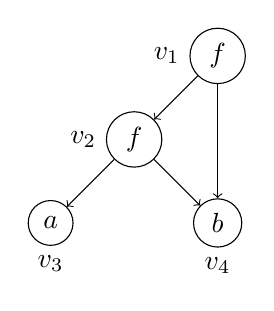
\begin{tikzpicture}[node distance={15mm}, main/.style = {draw, circle}]
\node[main, label=left:$v_{1}$] (1) {$f$};
\node[main, label=left:$v_{2}$] (2) [below left of=1] {$f$};
\node[main, label=below:$v_{3}$] (3) [below left of=2] {$a$};
\node[main, label=below:$v_{4}$] (4) [below right of=2] {$b$};
\draw[->] (1) -- (2);
\draw[->] (2) -- (3);
\draw[->] (2) -- (4);
\draw[->] (1) -- (4);
\end{tikzpicture}
\end{figure}

For a vertex $v$, we will denote by $\lambda(v)$ its label, $\delta(v)$ its outdegree and $Child(v, i)$ its $i$-th child.

Next, we will keep a data structure that is capable of representing a set of disjoint sets of vertices. Each one of these disjoint sets represents a class in an equivalence relation, where every vertex in the same class is known to be equal. This data structure must also be able to check whether two vertices are on the same class and to join two classes. An example of structure with such capabilities is~\cite{union_find}.

Initially, each term is only equal to itself. Then, for each equality $t_{1} = t_{2}$ in $S$ we will use the procedure \textit{MergeCong} presented below to merge the vertices $v_{1}$ and $v_{2}$ that correspond to $t_{1}$ and $t_{2}$:

\renewcommand{\algorithmicforall}{\textbf{for each}}
\MakeRobust{\Call}

\begin{algorithm}[H]
\caption{Merge with Congruence}~\label{merge_cong}
\begin{algorithmic}[1]
  \Function{MergeCong}{$v_{1}$, $v_{2}$}
  \If{\Call{SameClasses}{$v_{1}$, $v_{2}$}}
    \State\Return
  \EndIf
  \State Let $v_{1}^{*}$ and $v_{2}^{*}$ be the equivalence classes of $v_{1}$ and $v_{2}$.
  \State Let $P_{v_{1}^{*}}$ be the set of all predecessors of all vertices in $v_{1}^{*}$
  \State Let $P_{v_{2}^{*}}$ be the set of all predecessors of all vertices in $v_{2}^{*}$
  \State\Call{Merge}{$v_{1}$, $v_{2}$}
  \ForAll{$u_{1} \in P_{v_{1}^{*}}$ and $u_{2} \in P_{v_{2}^{*}}$}
    \If{\Call{IsCongruent}{$u_{1}$, $u_{2}$}}
      \State\Call{MergeCong}{$u_{1}$, $u_{2}$}
    \EndIf
  \EndFor
  \EndFunction
\end{algorithmic}
\end{algorithm}

\begin{algorithm}[H]
\caption{Check Congruence Condition}~\label{cong_cond}
\begin{algorithmic}[1]
  \Function{IsCongruent}{$v_{1}$, $v_{2}$}
  \If{$\lambda(v_{1}) \neq \lambda(v_{2})$ or $\delta(v_{1}) \neq \delta(v_{2})$}
    \State\Return~$false$
  \EndIf
  \For{$i = 1$ to $\delta(v_{1})$}
  \If{$\neg$ \Call{SameClasses}{\Call{Child}{$v_{1}$, $i$}, \Call{Child}{$v_{2}$, $i$}}}
      \State\Return $false$
    \EndIf
  \EndFor
  \State\Return $true$
  \EndFunction
\end{algorithmic}
\end{algorithm}

Notice that, when we process an equality $t_{1} = t_{2}$, we also have to propagate this information to any other terms that are using $t_{1}$ and $t_{2}$ as parameters (e.g.~if we have $f(t_{1})$ and $f(t_{2})$ as terms, we must also merge their classes). That's why we recursively call \textit{MergeCong} on line 11.

Once this process is done, we can check whether any pair of terms $t_{1}$ and $t_{2}$ is currently equal to each other by checking whether their corresponding vertices $v_{1}$ and $v_{2}$ are on the same equivalence class (i.e.\ checking whether $Find(v_{1}) = Find(v_{2})$). Therefore, we can use this fact to solve our original problem of checking if the equality $e$ follows from the conjunction of the equalities in $S$.

\subsubsection{Linear Arithmetic}

The second theory that we will be interested in this work is the theory of Linear Arithmetic. A term in this theory is an expression of the form:
\begin{center}
  $\mathlarger{\sum}_{i = 1}^{n} a_{i} x_{i} \bowtie b$
\end{center}

Where each $a_{i}$ and $b$ are constants ranging over rationals, each $x_{i}$ is a variable and $\bowtie$ is one of $\le$, $<$, $=$, $>$ or $\ge$. If we allow variables to range only over integers, we have the Linear Integer Arithmetic theory, which was described in terms of MSFOL in Example~\ref{ex:lia}. If we allow variables to range over rationals, we have the Linear Real Arithmetic (LRA) theory, which can be described using MSFOL in almost the same way, only changing $\mathcal{S}_{S}$ to $\{\mathbb{Q}\}$. \tom{we don't need to include rational constants in $\mathcal{S}_{F}$, right?}

We will now review the method presented in~\cite{simplex_dpllt} for checking whether a given set of atoms in this theory is satisfiable

For instance, let the set of those atoms be $\Phi := \{x - y \ge 3, x - y \le 10, x \ge 5, x - 2y < 6\}$. The first step is to, for each atom $t_{i} \bowtie b_{i} \in \Phi$ which does not have a single variable on the left side, create a new variable $s_{i}$. Then, we will define two new sets of atoms: $\Phi_{A}$, such that it's atoms are all of the form $s_{i} = t_{i}$, that is, they state the equality between the new variables and the corresponding terms, and $\Phi'$, that has all the atoms in $\Phi$ but with each term $t_{i}$ substituted by $s_{i}$. From our original set $\Phi$ we would define $\Phi_{A} := \{s_{1} = x - y, s_{2} = x - 2y\}$ and $\Phi' := \{s_{1} \ge 3\, s_{1} \le 10, x \ge 5, s_{2} < 6\}$. It is easy to see that $\Phi$ and $\Phi_{A} \wedge \Phi'$ are equisatisfiable.

Next we will represent the restrictions in $\Phi_{A}$ as $Ax = 0$, where $A$ is a matrix and $x$ is a vector with all the variables in the problem (including the ones we added). If the original problem had $n$ variables and we added $m$ new ones, the matrix $A$ will have dimensions $m$ and $m + n$. In our example, we would have the following:

\begin{center}
$
A :=
\begin{bmatrix}
  -1 & 1 & 1 & 0 \\
  -1 & 2 & 0 & 1
\end{bmatrix}
x :=
\begin{bmatrix}
  x & y & s_{1} & s_{2}
\end{bmatrix}^{T}
$
\end{center}

Now our problem is reduced to finding a vector $x$ that satisfies $Ax = 0$ and respects all restrictions in $\Psi'$, which are all of the form $v_{i} \bowtie b_{i}$. For now, we will assume that there is no strict inequalities in $\Psi'$ and rewrite it's restrictions as $l_{i} \le v_{i} \le r_{i}$, where $l_{i}$ will be $-\infty$ if there is no lower restriction on $v_{i}$ and $r_{i}$ will be $+\infty$ if there is no upper restriction on $v_{i}$.

\subsection{Proofs in cvc5}

\begin{itemize}
  \item Resolution tree (cite Rob65 from smtcoq to say that it is complete)
\end{itemize}

\subsection{Applications}

Given a program and a formal specification of some property related to the program, it is often \tom{always?} the case that we can express the proposition that asserts that the program satisfy the property as an SMT instance. For instance, consider the well known \textit{abs} function, that takes an integer and returns its absolute value. The usual way to implement it is through a branch that checks whether the input variable is positive or negative. In case it is positive, its own value is returned. Otherwise, the value multiplied by $-1$ is returned:

\begin{algorithm}[H]
\caption{Original Absolute Function}~\label{originalAbs}
\begin{algorithmic}[1]
\Function{abs}{x}
\If{$x < 0$}
  \State\Return$-x$
\Else
  \State\Return$x$
\EndIf
\EndFunction
\end{algorithmic}
\end{algorithm}

In program analysis, it is quite useful to eliminate branches from programs since this action completely removes one possible path that the flow of the program can take, simplifying it's analysis (besides optimizing it's performance). Obviously, this operation must be done with caution to not modify the original behavior of the program. In his book~\cite{hacker_delight}, Henry Warren proposes an alternative implementation for the \textit{abs} function which does not have branches:

\begin{algorithm}[H]
\caption{Branchless Absolute Function}~\label{branchlessAbs}
\begin{algorithmic}[1]
\Function{abs'}{x}
  \State $y \gets x >> 31$
  \State \Return $(x \bigoplus y) - y$
\EndFunction
\end{algorithmic}
\end{algorithm}

Where $\bigoplus$ represents the bitwise xor operation. We can design an instance of the SMT problem that asserts that both implementations produce the same output, when given the same input. We present the instance written in SMT-LIB~\cite{smtlib}, a standardized syntax for representing SMT problems:

\begin{minted}[linenos]{smtlib2.py -x}
(set-logic QF_BV)
(declare-const x (_ BitVec 32))
(declare-const result1 (_ BitVec 32))
(assert (= result1 (ite (bvslt x #x00000000) (bvneg x) x)))
(declare-const y (_ BitVec 32))
(declare-const result2 (_ BitVec 32))
(assert (= y (bvashr x (_ bv31 32))))
(assert (= result2 (bvsub (bvxor x y) y)))
(assert (distinct result1 result2))
(check-sat)
\end{minted}

First, we set the combination of theories that will be used in this problem. In our case, we will be using \textit{QF\_BV}, which stands for quantifier free bitvectors. This means that this instance of the problem is not allowed to use quantifiers and is allowed to declare and use variables living in the Bitvector sort, as well as operations over this sort. Bitvectors are fixed-length arrays of bits. They are useful for representing machine integers, as they can simulate their semantics.

Next, in lines 2 and 3, we define two constants, both from the sort \textit{BitVec 32} (arrays of 32 bits): \textit{x} and \textit{result1}. The first one represents the input value from the original \textit{abs} function, and the second one, the result produced by that function. We then have to add an assertion in line 4 that binds the variable \textit{result1} to the output of the function \textit{abs} in terms of \textit{x}. We translate the branch from the pseudocode as the \textit{ite} operator, the comparison as the \textit{bvslt} operator and the multiplication by -1 as the \textit{bvneg} operation. In lines 5 to 8 we repeat the process to define \textit{y} and \textit{result2}, which corresponds to the result of the branchless \textit{abs} function. Finally, we assert that \textit{result1} and \textit{result2} must be different in line 9. If this problem is satisfiable, then there is a value for \textit{x} which produces different values in each function. If it is unsatisfiable, then we can be sure that no such value exists, therefore, both functions are equivalent. Note that we are not verifying that the actual code of the functions are equivalent, just an abstraction over it's implementation.

% Given that we have very efficient systems to solve such problems, which will be introduced later, the possibility of formally verifying programs using this technology is quite promising. Indeed, \tom{pegar referencias do paper do leonardo (https://fm.csl.sri.com/SSFT14/smt-application-chapter.pdf)}
%

% \begin{itemize}
%   \item revolucao sat
%   \item representar propriedades de programas como problemas smt
%   \item geracao de casos de teste
%   \item geracao de programas
%   \item F*, Dafny
% \end{itemize}
